\documentclass[12pt, xcolor=dvipsnames,svgnames,x11names]{article}

% ============================================================
% Homework identity
% ============================================================
\newcommand{\hw}{Classwork 7}
\newcommand{\hwtopic}{Simple Linear Regression in One Variable}
\newcommand{\duedate}{September 30, 2026, 11:59 PM}
\newcommand{\totalpoints}{50}
\newcommand{\hwturnin}{cw07}

\usepackage[fleqn]{nccmath}

\usepackage{tikz}
\usepackage{pgfplots}
\usepackage{minted}





\def\m@th{\normalcolor\mathsurround\z@}

\setlength{\parskip}{\baselineskip}%
\setlength{\parindent}{0pt}%

\def\e{{\textrm{e}}}
\def\d{\textrm{d}}
\def\T{{\textsf{T}}}
\def\sech{{\textrm{sech}}}
\def\x{{\mathbf x}}

\def\++{{$^{++}$}}

\def\Abb{{\mathbb A}}
\def\Bbb{{\mathbb B}}
\def\Cbb{{\mathbb C}}
\def\Dbb{{\mathbb D}}
\def\Ebb{{\mathbb E}}
\def\Fbb{{\mathbb F}}
\def\Gbb{{\mathbb G}}
\def\Hbb{{\mathbb H}}
\def\Ibb{{\mathbb I}}
\def\Jbb{{\mathbb J}}
\def\Kbb{{\mathbb K}}
\def\Lbb{{\mathbb L}}
\def\Mbb{{\mathbb M}}
\def\Nbb{{\mathbb N}}
\def\Obb{{\mathbb O}}
\def\Pbb{{\mathbb P}}
\def\Qbb{{\mathbb Q}}
\def\Rbb{{\mathbb R}}
\def\Sbb{{\mathbb S}}
\def\Tbb{{\mathbb T}}
\def\Ubb{{\mathbb U}}
\def\Vbb{{\mathbb V}}
\def\Wbb{{\mathbb W}}
\def\Xbb{{\mathbb X}}
\def\Ybb{{\mathbb Y}}
\def\Zbb{{\mathbb Z}}



\def\Acal{{\mathcal A}}
\def\Bcal{{\mathcal B}}
\def\Ccal{{\mathcal C}}
\def\Dcal{{\mathcal D}}
\def\Ecal{{\mathcal E}}
\def\Fcal{{\mathcal F}}
\def\Gcal{{\mathcal G}}
\def\Hcal{{\mathcal H}}
\def\Ical{{\mathcal I}}
\def\Jcal{{\mathcal J}}
\def\Kcal{{\mathcal K}}
\def\Lcal{{\mathcal L}}
\def\Mcal{{\mathcal M}}
\def\Ncal{{\mathcal N}}
\def\Ocal{{\mathcal O}}
\def\Pcal{{\mathcal P}}
\def\Qcal{{\mathcal Q}}
\def\Rcal{{\mathcal R}}
\def\Scal{{\mathcal S}}
\def\Tcal{{\mathcal T}}
\def\Ucal{{\mathcal U}}
\def\Vcal{{\mathcal V}}
\def\Wcal{{\mathcal W}}
\def\Xcal{{\mathcal X}}
\def\Ycal{{\mathcal Y}}
\def\Zcal{{\mathcal Z}}

\def\abf{{\mathbf a}}
\def\bbf{{\mathbf b}}
\def\cbf{{\mathbf c}}
\def\dbf{{\mathbf d}}
\def\ebf{{\mathbf e}}
\def\fbf{{\mathbf f}}
\def\gbf{{\mathbf g}}
\def\hbf{{\mathbf h}}
\def\ibf{{\mathbf i}}
\def\jbf{{\mathbf j}}
\def\kbf{{\mathbf k}}
\def\lbf{{\mathbf l}}
\def\mbf{{\mathbf m}}
\def\nbf{{\mathbf n}}
\def\obf{{\mathbf o}}
\def\pbf{{\mathbf p}}
\def\qbf{{\mathbf q}}
\def\rbf{{\mathbf r}}
\def\sbf{{\mathbf s}}
\def\tbf{{\mathbf t}}
\def\ubf{{\mathbf u}}
\def\vbf{{\mathbf v}}
\def\wbf{{\mathbf w}}
\def\xbf{{\mathbf x}}
\def\ybf{{\mathbf y}}
\def\zbf{{\mathbf z}}

\def\Abf{{\mathbf A}}
\def\Bbf{{\mathbf B}}
\def\Cbf{{\mathbf C}}
\def\Dbf{{\mathbf D}}
\def\Ebf{{\mathbf E}}
\def\Fbf{{\mathbf F}}
\def\Gbf{{\mathbf G}}
\def\Hbf{{\mathbf H}}
\def\Ibf{{\mathbf I}}
\def\Jbf{{\mathbf J}}
\def\Kbf{{\mathbf K}}
\def\Lbf{{\mathbf L}}
\def\Mbf{{\mathbf M}}
\def\Nbf{{\mathbf N}}
\def\Obf{{\mathbf O}}
\def\Pbf{{\mathbf P}}
\def\Qbf{{\mathbf Q}}
\def\Rbf{{\mathbf R}}
\def\Sbf{{\mathbf S}}
\def\Tbf{{\mathbf T}}
\def\Ubf{{\mathbf U}}
\def\Vbf{{\mathbf V}}
\def\Wbf{{\mathbf W}}
\def\Xbf{{\mathbf X}}
\def\Ybf{{\mathbf Y}}
\def\Zbf{{\mathbf Z}}

\def\phat{{\hat p}}

\usepackage{amsmath}
\DeclareMathOperator*{\argmax}{arg\,max}
\DeclareMathOperator*{\argmin}{arg\,min}

\def\xbar{{\overline x}}
\def\ybar{{\overline y}}
\def\e{{\textrm{e}}}
\def\d{\textrm{d}}
\def\T{{\textsf{T}}}
\def\sech{{\textrm{sech}}}
\def\x{{\mathbf x}}

\def\++{{$^{++}$}}

\def\Abb{{\mathbb A}}
\def\Bbb{{\mathbb B}}
\def\Cbb{{\mathbb C}}
\def\Dbb{{\mathbb D}}
\def\Ebb{{\mathbb E}}
\def\Fbb{{\mathbb F}}
\def\Gbb{{\mathbb G}}
\def\Hbb{{\mathbb H}}
\def\Ibb{{\mathbb I}}
\def\Jbb{{\mathbb J}}
\def\Kbb{{\mathbb K}}
\def\Lbb{{\mathbb L}}
\def\Mbb{{\mathbb M}}
\def\Nbb{{\mathbb N}}
\def\Obb{{\mathbb O}}
\def\Pbb{{\mathbb P}}
\def\Qbb{{\mathbb Q}}
\def\Rbb{{\mathbb R}}
\def\Sbb{{\mathbb S}}
\def\Tbb{{\mathbb T}}
\def\Ubb{{\mathbb U}}
\def\Vbb{{\mathbb V}}
\def\Wbb{{\mathbb W}}
\def\Xbb{{\mathbb X}}
\def\Ybb{{\mathbb Y}}
\def\Zbb{{\mathbb Z}}



\def\Acal{{\mathcal A}}
\def\Bcal{{\mathcal B}}
\def\Ccal{{\mathcal C}}
\def\Dcal{{\mathcal D}}
\def\Ecal{{\mathcal E}}
\def\Fcal{{\mathcal F}}
\def\Gcal{{\mathcal G}}
\def\Hcal{{\mathcal H}}
\def\Ical{{\mathcal I}}
\def\Jcal{{\mathcal J}}
\def\Kcal{{\mathcal K}}
\def\Lcal{{\mathcal L}}
\def\Mcal{{\mathcal M}}
\def\Ncal{{\mathcal N}}
\def\Ocal{{\mathcal O}}
\def\Pcal{{\mathcal P}}
\def\Qcal{{\mathcal Q}}
\def\Rcal{{\mathcal R}}
\def\Scal{{\mathcal S}}
\def\Tcal{{\mathcal T}}
\def\Ucal{{\mathcal U}}
\def\Vcal{{\mathcal V}}
\def\Wcal{{\mathcal W}}
\def\Xcal{{\mathcal X}}
\def\Ycal{{\mathcal Y}}
\def\Zcal{{\mathcal Z}}

\def\abf{{\mathbf a}}
\def\bbf{{\mathbf b}}
\def\cbf{{\mathbf c}}
\def\dbf{{\mathbf d}}
\def\ebf{{\mathbf e}}
\def\fbf{{\mathbf f}}
\def\gbf{{\mathbf g}}
\def\hbf{{\mathbf h}}
\def\ibf{{\mathbf i}}
\def\jbf{{\mathbf j}}
\def\kbf{{\mathbf k}}
\def\lbf{{\mathbf l}}
\def\mbf{{\mathbf m}}
\def\nbf{{\mathbf n}}
\def\obf{{\mathbf o}}
\def\pbf{{\mathbf p}}
\def\qbf{{\mathbf q}}
\def\rbf{{\mathbf r}}
\def\sbf{{\mathbf s}}
\def\tbf{{\mathbf t}}
\def\ubf{{\mathbf u}}
\def\vbf{{\mathbf v}}
\def\wbf{{\mathbf w}}
\def\xbf{{\mathbf x}}
\def\ybf{{\mathbf y}}
\def\zbf{{\mathbf z}}

\def\Abf{{\mathbf A}}
\def\Bbf{{\mathbf B}}
\def\Cbf{{\mathbf C}}
\def\Dbf{{\mathbf D}}
\def\Ebf{{\mathbf E}}
\def\Fbf{{\mathbf F}}
\def\Gbf{{\mathbf G}}
\def\Hbf{{\mathbf H}}
\def\Ibf{{\mathbf I}}
\def\Jbf{{\mathbf J}}
\def\Kbf{{\mathbf K}}
\def\Lbf{{\mathbf L}}
\def\Mbf{{\mathbf M}}
\def\Nbf{{\mathbf N}}
\def\Obf{{\mathbf O}}
\def\Pbf{{\mathbf P}}
\def\Qbf{{\mathbf Q}}
\def\Rbf{{\mathbf R}}
\def\Sbf{{\mathbf S}}
\def\Tbf{{\mathbf T}}
\def\Ubf{{\mathbf U}}
\def\Vbf{{\mathbf V}}
\def\Wbf{{\mathbf W}}
\def\Xbf{{\mathbf X}}
\def\Ybf{{\mathbf Y}}
\def\Zbf{{\mathbf Z}}

\def\phat{{\hat p}}
\def\what{{\hat w}}
\def\yhat{{\hat y}}


\newcommand{\answer}{
    \fcolorbox{orange}{PapayaWhip}{
\begin{minipage}{\textwidth}
        \textbf{Answer}
    \end{minipage}
}
}

\newcommand{\codeoutput}[1]{
Output:\\\vspace{5px}
    \fcolorbox{orange}{WhiteSmoke}{
\begin{minipage}{\textwidth}
        { \color{DodgerBlue} 
        
        
       \texttt{#1}
       }
    \end{minipage}
}
}


\newcommand{\orangebox}[1]{
    \fcolorbox{orange}{white}{
\begin{minipage}{\textwidth}
       {\color{MidnightBlue} 
       #1
       }
    \end{minipage}
}
}


\definecolor{lightapricot}{rgb}{0.99, 0.84, 0.69}
\definecolor{lightblue}{rgb}{0.68, 0.85, 0.90}
\definecolor{blanchedalmond}{rgb}{1.0, 0.92, 0.8}
\definecolor{blizzardblue}{rgb}{0.67, 0.9, 0.93}
\definecolor{blond}{rgb}{0.98, 0.94, 0.75}
\definecolor{babyblueeyes}{rgb}{0.63, 0.79, 0.95}
\definecolor{babypink}{rgb}{0.96, 0.76, 0.76}
\definecolor{bananamania}{rgb}{0.98, 0.91, 0.71}
\definecolor{beaublue}{rgb}{0.74, 0.83, 0.9}
\definecolor{antiquewhite}{rgb}{0.98, 0.92, 0.84}
\definecolor{anti-flashwhite}{rgb}{0.95, 0.95, 0.96}
\definecolor{brightlavender}{rgb}{0.75, 0.58, 0.89}
\definecolor{brightube}{rgb}{0.82, 0.62, 0.91}
\definecolor{brilliantlavender}{rgb}{0.96, 0.73, 1.0}
\definecolor{lightcerulean}{rgb}{0.11, 0.67, 0.84}
\definecolor{cpeyellow}{HTML}{F5F5DC}                 % Beige (much softer)
\definecolor{powderGreen}{HTML}{F0F8E8}               % Very pale mint


% Darker versions of the original colors
\definecolor{deepapricot}{rgb}{0.85, 0.65, 0.45}        % darker lightapricot
\definecolor{deepblue}{rgb}{0.45, 0.65, 0.75}           % darker lightblue
\definecolor{toastedalmond}{rgb}{0.85, 0.75, 0.60}      % darker blanchedalmond
\definecolor{stormblue}{rgb}{0.45, 0.70, 0.75}          % darker blizzardblue
\definecolor{goldenrod}{rgb}{0.80, 0.75, 0.50}          % darker blond
\definecolor{royalblue}{rgb}{0.40, 0.60, 0.80}          % darker babyblueeyes
\definecolor{rosewood}{rgb}{0.75, 0.45, 0.45}           % darker babypink
\definecolor{mustardyellow}{rgb}{0.80, 0.70, 0.45}      % darker bananamania
\definecolor{navyblue}{rgb}{0.50, 0.60, 0.70}           % darker beaublue
\definecolor{antiquetan}{rgb}{0.80, 0.70, 0.60}         % darker antiquewhite
\definecolor{silvergray}{rgb}{0.75, 0.75, 0.80}         % darker anti-flashwhite
\definecolor{darklavender}{rgb}{0.55, 0.35, 0.70}       % darker brightlavender
\definecolor{deepube}{rgb}{0.65, 0.40, 0.75}            % darker brightube
\definecolor{plumviolet}{rgb}{0.75, 0.50, 0.85}         % darker brilliantlavender
\definecolor{deepcerulean}{rgb}{0.08, 0.45, 0.65}       % darker lightcerulean

\definecolor{roseRed}{HTML}{e20047}
\definecolor{coolGray}{HTML}{474747} % Neutral gray to contrast roseRed
\definecolor{mocha}{HTML}{a47864}
\definecolor{sage}{HTML}{8a9a5b}
\definecolor{dustyblue}{HTML}{6e8ca0}
\definecolor{terracotta}{HTML}{c87f5b}
\definecolor{lavender}{HTML}{9d8bb0}
\definecolor{darkmocha}{HTML}{7a5a4b}
\definecolor{darksage}{HTML}{667244}
\definecolor{darkdustyblue}{HTML}{526878}
\definecolor{darkterracotta}{HTML}{9e6347}
\definecolor{darklavender}{HTML}{766688}
\definecolor{winery}{HTML}{7e212a}

\usepackage{sectsty}
\sectionfont{\color{darklavender}}  % sets colour of sections
\subsectionfont{\color{plumviolet}}  % sets colour of sections
\subsubsectionfont{\color{deepube}}  % sets colour of sections

\usepackage{xcolor}
%\usepackage{universityos}
\usepackage{xspace}
\usepackage{url}
\usepackage[colorlinks=true,bookmarks=false,linkcolor=black,urlcolor=blue,citecolor=black]{hyperref}
\usepackage{fancyhdr}
\usepackage[top=1in,bottom=1in,left=1in,right=1in]{geometry}
\usepackage{multicol}
\usepackage{pgfplots}
\usetikzlibrary{circuits.logic.US}
% \usepackage{tgschola}
\let\temp\rmdefault
\usepackage{mathpazo}
\let\rmdefault\temp

\usepackage{eso-pic}



\usetikzlibrary{calc}
\usepackage{circuitikz}



\usepackage[many]{tcolorbox}
\setlength{\parindent}{0pt}
\setlength{\parskip}{4pt}%

\newcommand{\coursenumber}{CPE 486/586}
\newcommand{\courseyear}{2025\xspace}
\newcommand{\coursedatetime}{Tue/Thur 11:20 AM -- 12:40 PM\xspace}
\newcommand{\coursetitle}{Machine Learning for Engineering Applications\xspace}
\newcommand{\courseterm}{Fall, \courseyear}
\newcommand{\instructorname}{Rahul Bhadani\xspace}
\newcommand{\instructoremail}{\href{mailto:rahul.bhadani@uah.edu}{rahul.bhadani@uah.edu}}
\newcommand{\instructoroffice}{ENG 217-H\xspace}




\usepackage{design}

\pagestyle{fancy}

\lhead{\footnotesize{\coursenumber, \courseterm}}
\chead{}
\rhead{\footnotesize{\emph{\hw}}}
\lfoot{\footnotesize{\instructorname}}
\cfoot{\footnotesize{\thepage}}
\rfoot{\footnotesize{\textit{Last Revised:~\today}}\\ \footnotesize{The University of Alabama in Huntsville}}
\renewcommand{\headrulewidth}{0.1pt}
\renewcommand{\footrulewidth}{0.1pt}

\renewcommand{\thefootnote}{\fnsymbol{footnote}}


\renewcommand{\headrulewidth}{0.1pt}
\renewcommand{\footrulewidth}{0.1pt}

\renewcommand{\thefootnote}{\fnsymbol{footnote}}

\newcommand{\showanswers}{no}

\begin{document}


\date{Due: \duedate}

\maketitle


\section{Simple Linear Regression}
Consider the dataset that exhibits linear relationship between Units Sold in 1000 (predictor variable $x$), and profit in percentage ($y$):

\begin{tabular}{|c|c|}
\hline
\textbf{UnitSold\_in\_1000 $x_i$} & \textbf{Profits\_Pct $y_i$} \\
\hline
0.54 & 3.69 \\
\hline
0.72 & 4.58 \\
\hline
0.6 & 4.03 \\
\hline
0.54 & 3.67 \\
\hline
0.42 & 3.40 \\
\hline
0.64 & 4.03 \\
\hline
0.43 & 3.76 \\
\hline
0.89 & 4.61 \\
\hline
0.96 & 4.98 \\
\hline
0.38 & 2.89 \\
\hline
\end{tabular}

$n = 10$.

\bigskip

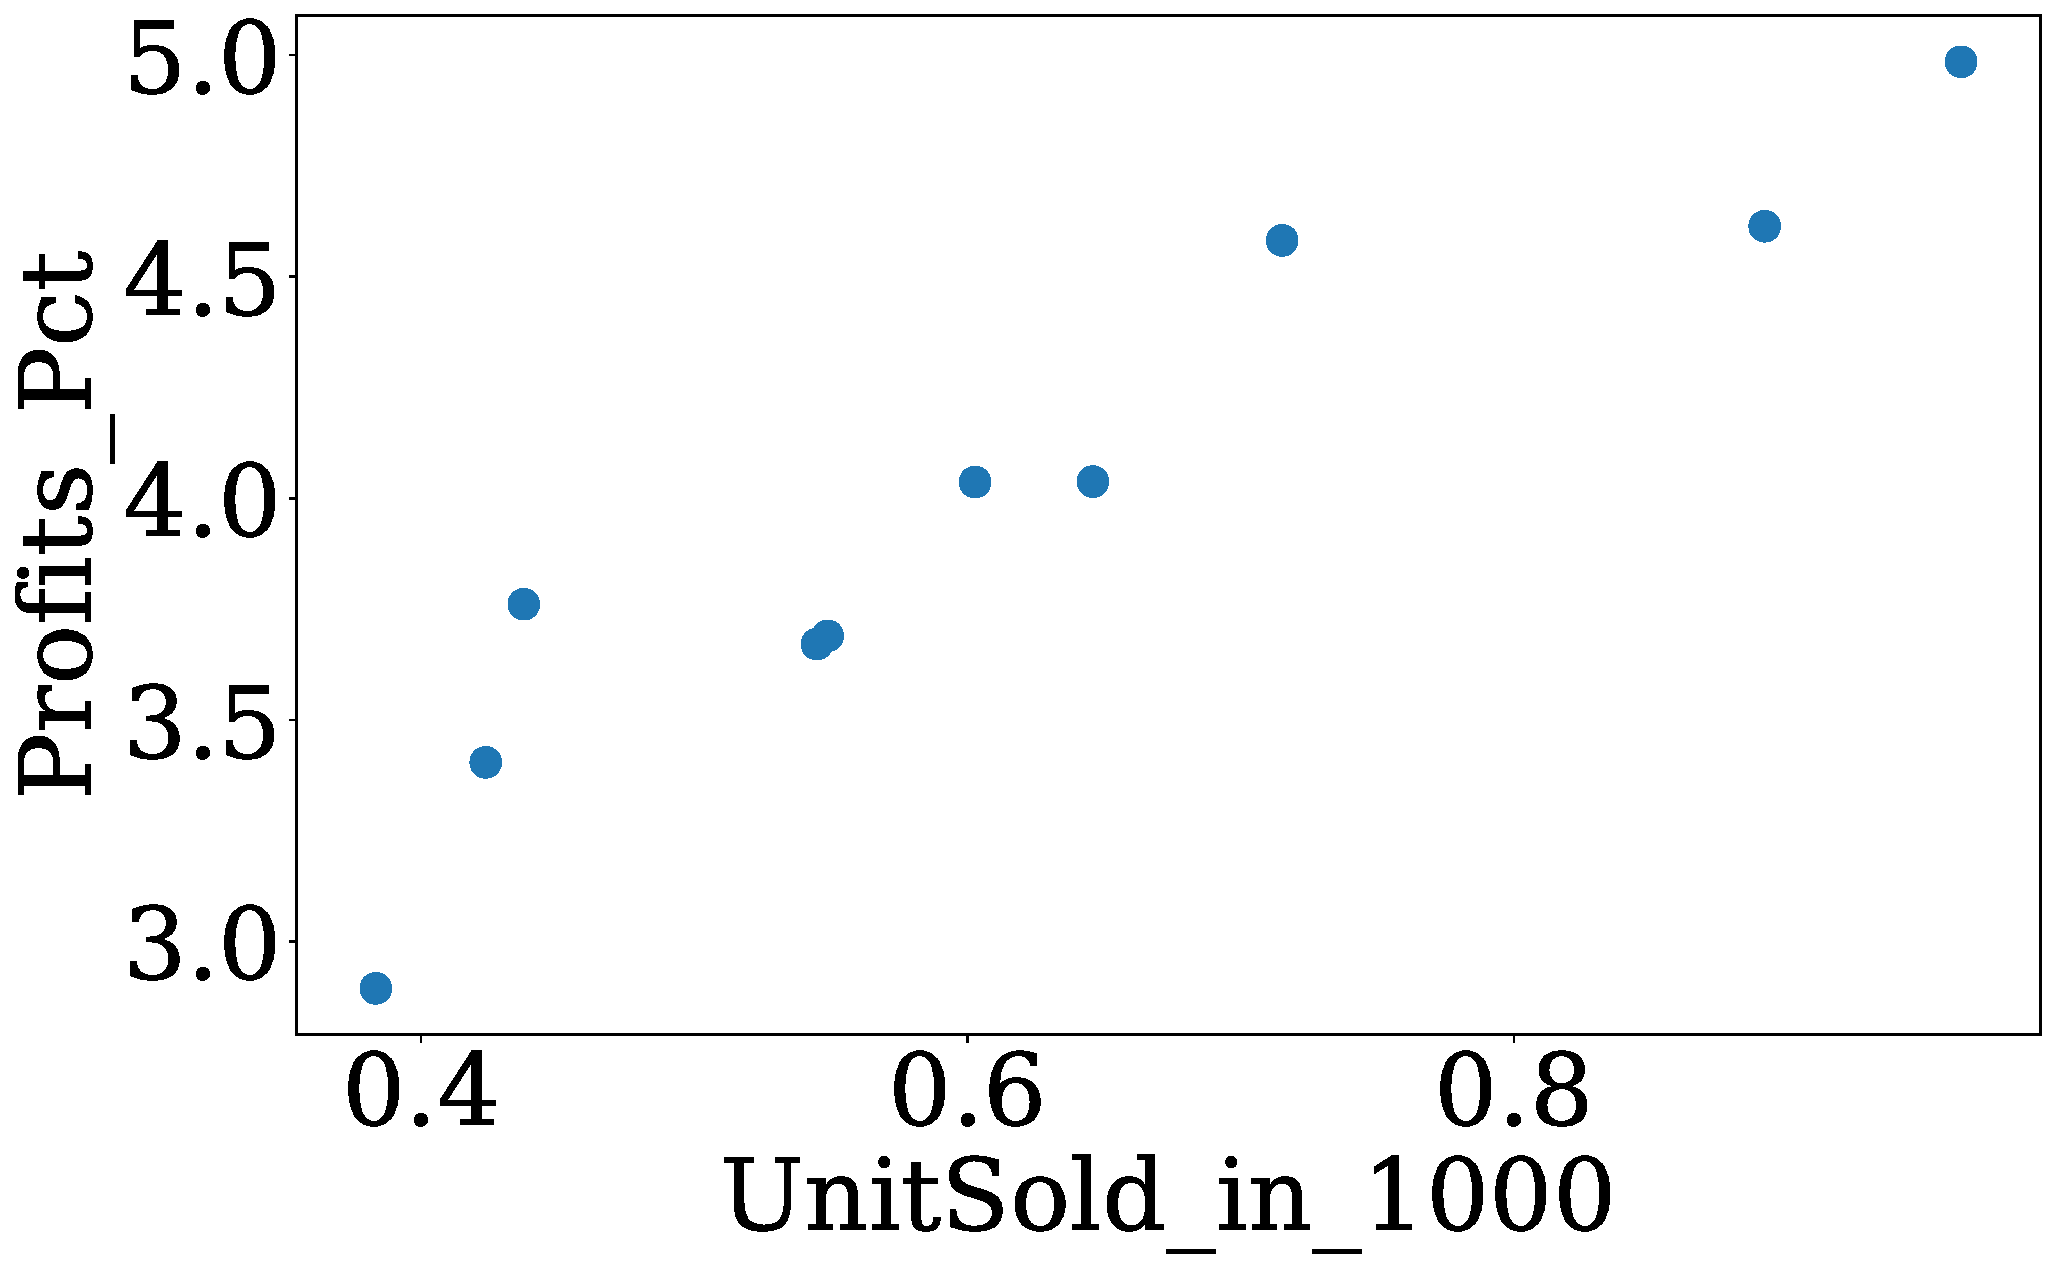
\includegraphics[width=0.65\textwidth]{../Lectures/figures/unitsold_profitsdata.pdf}

\newpage

\textbf{Calculate the following quantity ($\sum_{i=1}^{10}$ is shorthanded as $\sum$) (10 points):}

\begin{multicols}{3}
\begin{enumerate}
 \item \begin{equation*}
    \sum x_i = \vcenter{\hbox{\begin{tikzpicture}
    \draw (0,0) rectangle (75pt,75pt);
    \end{tikzpicture}}}
    \end{equation*}

\item \begin{equation*}
    \sum y_i = \vcenter{\hbox{\begin{tikzpicture}
    \draw (0,0) rectangle (75pt,75pt);
    \end{tikzpicture}}}
    \end{equation*}

    \item \begin{equation*}
    \xbar = \vcenter{\hbox{\begin{tikzpicture}
    \draw (0,0) rectangle (75pt,75pt);
    \end{tikzpicture}}}
    \end{equation*}

\item \begin{equation*}
    \ybar = \vcenter{\hbox{\begin{tikzpicture}
    \draw (0,0) rectangle (75pt,75pt);
    \end{tikzpicture}}}
    \end{equation*}

\item \begin{equation*}
     \sum (x_i -\xbar) = \vcenter{\hbox{\begin{tikzpicture}
    \draw (0,0) rectangle (75pt,75pt);
    \end{tikzpicture}}}
    \end{equation*}
    
\item \begin{equation*}
     \sum (y_i -\ybar) = \vcenter{\hbox{\begin{tikzpicture}
    \draw (0,0) rectangle (75pt,75pt);
    \end{tikzpicture}}}
    \end{equation*}

\item \begin{equation*}
     \sum (x_i -\xbar)^2 = \vcenter{\hbox{\begin{tikzpicture}
    \draw (0,0) rectangle (75pt,75pt);
    \end{tikzpicture}}}
    \end{equation*}

\item \begin{equation*}
     \sum (x_i y_i) = \vcenter{\hbox{\begin{tikzpicture}
    \draw (0,0) rectangle (75pt,75pt);
    \end{tikzpicture}}}
    \end{equation*}

\item \begin{equation*}
     \sum x_i^2 = \vcenter{\hbox{\begin{tikzpicture}
    \draw (0,0) rectangle (75pt,75pt);
    \end{tikzpicture}}}
    \end{equation*}

\item \begin{equation*}
     \sum y_i^2 = \vcenter{\hbox{\begin{tikzpicture}
    \draw (0,0) rectangle (75pt,75pt);
    \end{tikzpicture}}}
    \end{equation*}

\item \begin{equation*}
     \sum (x_i - \xbar) (y_i - \ybar) = \vcenter{\hbox{\begin{tikzpicture}
    \draw (0,0) rectangle (75pt,75pt);
    \end{tikzpicture}}}
    \end{equation*}
        
\end{enumerate}
\end{multicols}

In an ideal scenario, the data was obtained from a linear model $Y = Xw_1 + w_0$. The given data comes follows the $y_i = x_i w_1 + w_0 + \epsilon_i$ where $\epsilon_i$ is the error introduced by data gathering process such that $\epsilon_i \sim \Ncal(\mu= 0, \sigma=0.3)$. 

We will fit our data into the linear model $y_i=x_i w_1 + w_0$ with the hope of minimizing the cost function (or error):

\begin{equation}
    Q = \cfrac{1}{n}\sum_i (y_i -\yhat)^2
\end{equation}
where $\yhat = x_i \what_1 + \what_0$.

The least-square solution gives the normal equation by solving:

\begin{equation}
    \begin{aligned}
    \sum y_i & = n\what_0 + \what_1 \sum x_i\\
    \sum x_i y_i & = \what_0 \sum x_i + \what_1 \sum x_i^2
    \end{aligned}
\end{equation}

which gives 
\begin{equation}
    \what_1 = \cfrac{\sum_i (x_i - \xbar)(y_i - \ybar)}{\sum_i (x_i  - \xbar)^2} = \cfrac{\quad\quad\quad\quad\quad\quad\quad\quad\quad\quad\quad\quad\quad\quad\quad\quad\quad}{\quad\quad\quad\quad\quad\quad\quad\quad\quad\quad\quad\quad\quad\quad\quad\quad\quad} = \vcenter{\hbox{\begin{tikzpicture}
    \draw (0,0) rectangle (75pt,75pt);
    \end{tikzpicture}}}
\end{equation}

\textbf{(4 Points)}

and

\begin{equation}
    \what_0 = \ybar - \what_1 \xbar = \vcenter{\hbox{\begin{tikzpicture}
    \draw (0,0) rectangle (75pt,75pt);
    \end{tikzpicture}}} 
\end{equation}
\textbf{~~~(2 Points)}



Alternatively, we can take the derivative of the cost function which can be re-written as
\begin{equation}
    Q = \cfrac{1}{n} \sum ( y_i - (w_1x_i + w_0))^2
\end{equation}

Taking the partial derivative with respect to $w_1$ and $w_0$:

\begin{figure}[h]
\fbox{
\begin{minipage}{\linewidth}
\vspace{20pt}
\begin{fleqn}
\begin{equation}
\cfrac{\partial Q}{\partial w_1} = 
\end{equation}
\end{fleqn}
\vspace{150pt}
\end{minipage}
}
\textbf{~~~(5 Points)}
\end{figure}

\newpage

\begin{figure}[h]
\fbox{
\begin{minipage}{\linewidth}
\vspace{20pt}
\begin{fleqn}
\begin{equation}
\cfrac{\partial Q}{\partial w_0} = 
\end{equation}
\end{fleqn}
\vspace{150pt}
\end{minipage}
}
\textbf{~~~(5 Points)}

\end{figure}



Setting above to 0 gives the following set of equations:

\begin{equation}
    \begin{aligned}
        w_1 & = \frac{n(\sum_{i=1}^{n} x_i y_i) - (\sum_{i=1}^{n} x_i)(\sum_{i=1}^{n} y_i)}{n(\sum_{i=1}^{n} x_i^2) - (\sum_{i=1}^{n} x_i)^2}
        \\
        w_0 & = \frac{1}{n}(\sum_{i=1}^{n} y_i) - w_1 \frac{1}{n}(\sum_{i=1}^{n} x_i)
    \end{aligned}
\end{equation}

Putting the value in the above equations should give an estimated $\what_0$ and $\what_1$. Write down what you got in that Equation.


\begin{equation}
    \begin{aligned}
       \what_1 = 
    \end{aligned}
\end{equation}

\vspace{100pt}

\begin{equation}
    \begin{aligned}
       \what_0 = 
    \end{aligned}
\end{equation}


\vspace{100pt}
\textbf{~~~(5 Points)}


Using $\what_0$ and $\what_1$, we can obtain $\yhat_i$, the estimated response. Using estimated response and actual response, we can calculate Sum of Square Error (SSE) and Total Square Sum (SSTO) as:

\begin{equation}
\begin{aligned}
        \textrm{SSE} & = \sum (y_i - \yhat_i)^2 = \\
        \textrm{MSE} & = \cfrac{\textrm{SSE}}{n - 2} = \\
        \textrm{SSTO} & = \sum (y_i - \ybar)^2 = 
\end{aligned}
\end{equation}
\textbf{~~~(2 Points)}

Calculate the goodness of fit using the coefficient of determination $R^2$:


\begin{equation}
    R^2 = 1 - \cfrac{\textrm{SSE}}{\textrm{SSTO}} = 
\end{equation}
\textbf{~~~(2 Points)}


\begin{figure}[h]
\fbox{
\begin{minipage}{\linewidth}
\begin{fleqn}
\textbf{Based on the value of $R^2$ how good fit is the linear model on the given dataset?
}
\end{fleqn}
\vspace{100pt}

\end{minipage}
}
\textbf{~~~(2 Points)}
\end{figure}


Next, we calculate the standard deviation on the estimated coefficients or weight ($\what_1$, and $\what_0$).

\begin{figure}[h]
\fbox{
\begin{minipage}{\linewidth}
\vspace{20pt}
\begin{fleqn}
\begin{equation}
s^2[\what_1] = \cfrac{\textrm{MSE}}{\sum (x_i - \xbar)^2} = 
\end{equation}
\end{fleqn}
\vspace{100pt}
\end{minipage}
}
\textbf{~~~(2 Points)}
\end{figure}


\begin{figure}[h]
\fbox{
\begin{minipage}{\linewidth}
\vspace{20pt}
\begin{fleqn}
\begin{equation}
s^2[\what_0] = \textrm{MSE}\bigg( \cfrac{1}{n} + \cfrac{\xbar^2}{\sum (x_i - \xbar)^2} \bigg)= 
\end{equation}
\end{fleqn}
\vspace{100pt}
\end{minipage}
}
\textbf{~~~(2 Points)}
\end{figure}

Now, we need to calculate the 95\% confidence interval on the estimated $\what_1$ and $\what_0$ for which $\alpha = 0.05$ (use $t(0.975, 8) = 2.306$):


\begin{figure}[h]
\fbox{
\begin{minipage}{\linewidth}
\vspace{20pt}
\begin{fleqn}
\begin{equation}
\what_1 \pm t(1 - 0.05/2, 10-2)s[\what_1]
\end{equation}
\end{fleqn}
\vspace{100pt}
\end{minipage}
}
\textbf{~~~(2 Points)}
\end{figure}



\begin{figure}[h]
\fbox{
\begin{minipage}{\linewidth}
\vspace{20pt}
\begin{fleqn}
\begin{equation}
\what_0 \pm t(1 - 0.05/2, 10-2)s[\what_0]
\end{equation}
\end{fleqn}
\vspace{100pt}
\end{minipage}
}
\textbf{~~~(2 Points)}
\end{figure}


Now, consider a new data point $x_{new} = 0.47$ Units Sold (in 1000). Based on the linear regression model that we developed, what is the estimated/predicted profit percent for the given quantity \textbf{~~~(5 Points)}?

\end{document}